% Options for packages loaded elsewhere
\PassOptionsToPackage{unicode}{hyperref}
\PassOptionsToPackage{hyphens}{url}
\PassOptionsToPackage{dvipsnames,svgnames,x11names}{xcolor}
%
\documentclass[
  12pt,
]{interact}

\usepackage{amsmath,amssymb}
\usepackage{setspace}
\usepackage{iftex}
\ifPDFTeX
  \usepackage[T1]{fontenc}
  \usepackage[utf8]{inputenc}
  \usepackage{textcomp} % provide euro and other symbols
\else % if luatex or xetex
  \usepackage{unicode-math}
  \defaultfontfeatures{Scale=MatchLowercase}
  \defaultfontfeatures[\rmfamily]{Ligatures=TeX,Scale=1}
\fi
\usepackage{lmodern}
\ifPDFTeX\else  
    % xetex/luatex font selection
\fi
% Use upquote if available, for straight quotes in verbatim environments
\IfFileExists{upquote.sty}{\usepackage{upquote}}{}
\IfFileExists{microtype.sty}{% use microtype if available
  \usepackage[]{microtype}
  \UseMicrotypeSet[protrusion]{basicmath} % disable protrusion for tt fonts
}{}
\makeatletter
\@ifundefined{KOMAClassName}{% if non-KOMA class
  \IfFileExists{parskip.sty}{%
    \usepackage{parskip}
  }{% else
    \setlength{\parindent}{0pt}
    \setlength{\parskip}{6pt plus 2pt minus 1pt}}
}{% if KOMA class
  \KOMAoptions{parskip=half}}
\makeatother
\usepackage{xcolor}
\setlength{\emergencystretch}{3em} % prevent overfull lines
\setcounter{secnumdepth}{5}
% Make \paragraph and \subparagraph free-standing
\makeatletter
\ifx\paragraph\undefined\else
  \let\oldparagraph\paragraph
  \renewcommand{\paragraph}{
    \@ifstar
      \xxxParagraphStar
      \xxxParagraphNoStar
  }
  \newcommand{\xxxParagraphStar}[1]{\oldparagraph*{#1}\mbox{}}
  \newcommand{\xxxParagraphNoStar}[1]{\oldparagraph{#1}\mbox{}}
\fi
\ifx\subparagraph\undefined\else
  \let\oldsubparagraph\subparagraph
  \renewcommand{\subparagraph}{
    \@ifstar
      \xxxSubParagraphStar
      \xxxSubParagraphNoStar
  }
  \newcommand{\xxxSubParagraphStar}[1]{\oldsubparagraph*{#1}\mbox{}}
  \newcommand{\xxxSubParagraphNoStar}[1]{\oldsubparagraph{#1}\mbox{}}
\fi
\makeatother


\providecommand{\tightlist}{%
  \setlength{\itemsep}{0pt}\setlength{\parskip}{0pt}}\usepackage{longtable,booktabs,array}
\usepackage{calc} % for calculating minipage widths
% Correct order of tables after \paragraph or \subparagraph
\usepackage{etoolbox}
\makeatletter
\patchcmd\longtable{\par}{\if@noskipsec\mbox{}\fi\par}{}{}
\makeatother
% Allow footnotes in longtable head/foot
\IfFileExists{footnotehyper.sty}{\usepackage{footnotehyper}}{\usepackage{footnote}}
\makesavenoteenv{longtable}
\usepackage{graphicx}
\makeatletter
\def\maxwidth{\ifdim\Gin@nat@width>\linewidth\linewidth\else\Gin@nat@width\fi}
\def\maxheight{\ifdim\Gin@nat@height>\textheight\textheight\else\Gin@nat@height\fi}
\makeatother
% Scale images if necessary, so that they will not overflow the page
% margins by default, and it is still possible to overwrite the defaults
% using explicit options in \includegraphics[width, height, ...]{}
\setkeys{Gin}{width=\maxwidth,height=\maxheight,keepaspectratio}
% Set default figure placement to htbp
\makeatletter
\def\fps@figure{htbp}
\makeatother

\usepackage{booktabs}
\usepackage{longtable}
\usepackage{array}
\usepackage{multirow}
\usepackage{wrapfig}
\usepackage{float}
\usepackage{colortbl}
\usepackage{pdflscape}
\usepackage{tabu}
\usepackage{threeparttable}
\usepackage{threeparttablex}
\usepackage[normalem]{ulem}
\usepackage{makecell}
\usepackage{xcolor}
\usepackage{orcidlink}
\makeatletter
\@ifpackageloaded{caption}{}{\usepackage{caption}}
\AtBeginDocument{%
\ifdefined\contentsname
  \renewcommand*\contentsname{Table of contents}
\else
  \newcommand\contentsname{Table of contents}
\fi
\ifdefined\listfigurename
  \renewcommand*\listfigurename{List of Figures}
\else
  \newcommand\listfigurename{List of Figures}
\fi
\ifdefined\listtablename
  \renewcommand*\listtablename{List of Tables}
\else
  \newcommand\listtablename{List of Tables}
\fi
\ifdefined\figurename
  \renewcommand*\figurename{Figure}
\else
  \newcommand\figurename{Figure}
\fi
\ifdefined\tablename
  \renewcommand*\tablename{Table}
\else
  \newcommand\tablename{Table}
\fi
}
\@ifpackageloaded{float}{}{\usepackage{float}}
\floatstyle{ruled}
\@ifundefined{c@chapter}{\newfloat{codelisting}{h}{lop}}{\newfloat{codelisting}{h}{lop}[chapter]}
\floatname{codelisting}{Listing}
\newcommand*\listoflistings{\listof{codelisting}{List of Listings}}
\makeatother
\makeatletter
\makeatother
\makeatletter
\@ifpackageloaded{caption}{}{\usepackage{caption}}
\@ifpackageloaded{subcaption}{}{\usepackage{subcaption}}
\makeatother

\ifLuaTeX
  \usepackage{selnolig}  % disable illegal ligatures
\fi
\usepackage[]{natbib}
\bibliographystyle{plainnat}
\usepackage{bookmark}

\IfFileExists{xurl.sty}{\usepackage{xurl}}{} % add URL line breaks if available
\urlstyle{same} % disable monospaced font for URLs
\hypersetup{
  pdftitle={My wonderful paper},
  pdfauthor={H. Sherry Zhang; Roger D. Peng},
  colorlinks=true,
  linkcolor={blue},
  filecolor={Maroon},
  citecolor={Blue},
  urlcolor={Blue},
  pdfcreator={LaTeX via pandoc}}


\title{My wonderful paper}
\author{H. Sherry Zhang$\textsuperscript{1}$, Roger D.
Peng$\textsuperscript{1}$}

\thanks{CONTACT: H. Sherry
Zhang. Email: \href{mailto:huize.zhang@austin.utexas.edu}{\nolinkurl{huize.zhang@austin.utexas.edu}}. Roger
D.
Peng. Email: \href{mailto:roger.peng@austin.utexas.edu}{\nolinkurl{roger.peng@austin.utexas.edu}}. }
\begin{document}
\captionsetup{labelsep=space}
\maketitle
\textsuperscript{1} Department of Statistics and Data
Sciences, University of Texas at Austin, Texas, United States
\begin{abstract}
In data analysis, unexpected results often prompt researchers to revisit
their procedures to identify potential issues. While experienced
researchers can typically diagnose problems by checking a few key
assumptions, others may struggle to identify the root causes. These
checked assumptions, or expectations, are typically informal, difficult
to trace, and rarely discussed in publications. In this paper, we
formalize these informal assumptions by framing them as binary
\emph{analysis validation check}. We then introduce a procedure to
quantify how violations of these checks may lead to unexpected results
in the analysis. The procedure relies on simulations of the original
data and evaluates boht accuracy and redundancy. Accuracy is calculated
through binary classification metric, while redundancy is measured using
mutual information. We demonstrate this approach with a toy example on
the fitness step count data and a generalized linear model exmaple
examining the effect of PM10 on mortality.
\end{abstract}


\setstretch{2}
README:

\begin{itemize}
\tightlist
\item
  \emph{Check for TODOs}
\item
  Literature review: Section \emph{diagnosing unexpected outcomes in
  data analysis}
\item
  \emph{Discussion} and \emph{Conclusion}
\item
  In Section \emph{Application}: provide more context on the
  PM10-mortality study and add reference of the {[}0, 0.005{]} PM10
  coefficient
\end{itemize}

\newpage

\section{Introduction}\label{introduction}

\begin{itemize}
\tightlist
\item
  TODO: emphasize trustworthy data science since it is the theme of the
  special issue
\end{itemize}

In data analysis, experienced researchers often rely on their prior
knowledge or domain expertise to quickly assess whether results align
with their expectations. When a result falls outside of this interval,
it prompts the researchers to investigate backwards on the data quality,
the analysis steps, or the assumptions made during the analysis process.
This mental process of where to diagnose unexpected outcomes is often
difficult to trace and discuss in publications. As a result, readers are
typically presented with the final outcomes of the analysis cycle where
the results and expectations are aligned -- achieved either by refining
the analysis or updating the expectations based on statistical evidence
\citep{grolemund_cognitive_2014}. These missing pieces of information
provides little guidance for diagnosing issues in the analysis when the
same methodology is applied to a new dataset that produces different
outcomes. Similarly, when researchers with different background
knowledge it becomes unclear whether discrepancies arise from differing
expectations or from the use of statistical techniques.

One might gain insight into analysts' thought process by speaking with
them directly or watching screencast videos they produce, such as,
TidyTuesday screencast videos. However, direct conversation are not
scalable and may not be feasible while creating educational videos
requires significant effort from the researchers. Ideally, there could
be a way to make these expectations explicit and accessible to others.
Even better, if the encoding is machine-readable, we could analyze these
expectations and learn from the analysis -- whether the checks also
apply to other researchers analyzing new data in the same context,
whether they reflect commo common practices in the field, or whether
they are specific to the data or analysis at hand.

In this paper, we conceptualize these internal expectations and
assumptions as \emph{analysis validation checks}, which allows us to
examine these assumptions made during analysis to diagnose unexpected
outcomes. We then introduce a procedure that provides a quantitative
emasure on how violations in a tree of checks, derived from individual
checks, will lead to an unexpected result. The procedure, based on
simulations of the original data, calculates accuracy and redundancy.
Accuracy is determined using binary classification metrics, precision
and recall, from a logic regression fit while redundancy is measured
using mutual information. The proposed workflow offers a numerical
guarantee that the analysis will produce the expected results, assuming
the data generating mechanism holds. {[}something about trustworthy data
science{]}

The rest of the paper is organized as follows:
Section~\ref{sec-lit-review} reviews the concept of diagnosing
unexpected outcomes and data quality checks. Section~\ref{sec-plan}
introduces the concept of analysis validation check, illustrated with a
toy example on fitness step count. Section~\ref{sec-method} describes
the procedure that quantify how checks combined in logical operators can
predict unexpected outcomes. Section~\ref{sec-pm10-mortality} applies
this procedure to examine the effect of PM10 on mortality in public
health in a generalized linear model. Section~\ref{sec-discussion}
discusses a few key considerations and Section~\ref{sec-conclusion}
concludes the paper.

\section{Literature review}\label{sec-lit-review}

\subsection{Diagnosing unexpected outcomes in data
analysis}\label{diagnosing-unexpected-outcomes-in-data-analysis}

\begin{itemize}
\item
  They shape how we interpret the results and assess whether they are
  consistent with existing knowledge or indicate the need for updates.
  \citep{grolemund_cognitive_2014}
\item
  \citep{peng_diagnosing_2021} describes three pedagogical exercises of
  introducing diagnosing unexpected outcome into a classroom setting.
\item
  what if the expectation is ``wrong''
\end{itemize}

\subsection{Data analysis checks}\label{data-analysis-checks}

A substantial body of literature has addressed the definition of data
quality \citep[more]{8642813} and developed frameworks, that includes
dimensions, attributes, and measures to evaluate and improve data
quality
\citep{cai2015challenges, wang1996beyond, 6204995, woodall2014classification}.
These frameworks are often used information system and database
management and support business decision-making in the industry. For
research purposes, high-quality data ensures the credibility of
scientific findings and supports reproducibility and reusability in
future studies {[}ref{]}. With the growing prevalence of open data in
scientific research, the consumers or users of the data typically are no
longer the data producers or collectors who have the full knowledge of
data in hand, prompting more interest towards the data quality checks in
the data analysis process. In R, there are some packages, like
\texttt{skimr} \citep{skimr} and \texttt{dataMaid} \citep{dataMaid},
provides basic data screening and reporting, while another class of
packages, e.g.~\texttt{assertr} \citep{assertr}, \texttt{validate}
\citep{validate}, and \texttt{pointblank} \citep{pointblank} focuses on
providing data validation tools, allowing users to define customized
data quality checks based on the applications.

\section{Analysis validation checks}\label{sec-plan}

\subsection{Framing expectations as
checks}\label{framing-expectations-as-checks}

Expectations represent our beliefs about certain aspects of the
analysis, independent of the analysis itself. When outcomes deviate from
these expectations, analysts often revisit the analysis cycle to
identify potential issues, refine methods, or revise assumptions.
Experienced analysts can typically identify issues quickly and correct
them on the spot, but they often do so without discussing the underlying
reasoning, making it harder for less experienced researchers to learn
and master these skills. Here, we introduce the concept of
\emph{analysis validation checks}, which frames these expectations or
assumptions as explicit checks that returns a TRUE or FALSE output given
the data analyzed at hand. Inspired by data validation checks
\citep{validate}, where ensure datasets meet expected format and
quality, analysis validation checks reverse the approach: they validate
the assumptions about the data necessary for the analysis to produce the
reported results. This allows the concept to encompass a broad range of
checks, such as data quality (i.e.~missing data, how the data is
structured), data distribution and outliers, bivariate and multivariate
relationships between variables, and contextual information. These
externalized checks provide insights into analysts' thoughts process
process and offer several benefits:

\begin{enumerate}
\def\labelenumi{\arabic{enumi})}
\tightlist
\item
  help students and junior researchers develop skills to diagnose
  unexpected analysis results,
\item
  serve as clear checkpoints to support replication or application of
  methods to (new) data,
\item
  align assumptions among researchers from different domain backgrounds,
  and
\item
  improve analysis transparency, reproducibility, and trustworthiness.
\end{enumerate}

\subsection{A toy example}\label{a-toy-example}

Consider a 30-day step count goal. Suppose you resolve to walk at least
8,000 steps each day, using an app to record your daily step count. Your
target average is 9,000 steps per day, with some ``lows'' day, where you
walk around 4,000 steps and ``high'' days where you reach about 12,000
steps. After 30 days, you check how many times your step count fall
below 8,000 and aim for no more than five days under this threshold.

To simulation this data, three normal distributions with different means
are used for the daily step counts: \(\mathcal{N}(4000, 200)\) for low
days, \(\mathcal{N}(12000, 200)\) for high days, and
\(\mathcal{N}(9000, 300)\) for typical days. The number of low and high
days can be simulated from a Poisson distribution with \(\lambda = 4\).
Figure~\ref{fig-step-count} displays the number of days with fewer than
8,000 steps across 300 simulated 30-day periods.

In this scenario, the outcome expectation is that the number of days
with a step count below 8,000 will be no more than five. To diagnose
potential reasons why this outcome expectation might fail, we can
establish a few plan expectations. For example, if the average step
count is too low, this may suggest there are too many low days,
potentially lead to an unexpected outcome. Similarly, we can also check
the quantile of the step count, if more than a third of the days fall
below 8,000, this could indicate an excess of low-count days.
Additionally, we may may expect the standard deviation of the step count
not to be overly large.

TODO: add one or two scenarios on why step count could go up or down: 1)
you take off your watch in the middle of the day, 2) have an workout

TODO: phrase it as Researcher measuring someone's step count rather than
measuring your own step count

These considerations yield the following three unit tests as plan
expectations:

\begin{itemize}
\tightlist
\item
  test1: the test fails if the mean step count is below 8,200
\item
  test2: the test fails if the 30th percentile of the step counts is
  below 8,200
\item
  test3: the test fails if the standard deviation of the step
  countsexceeds 2,500.
\end{itemize}

\phantomsection\label{cell-fig-step-count}
\begin{figure}[H]

\centering{

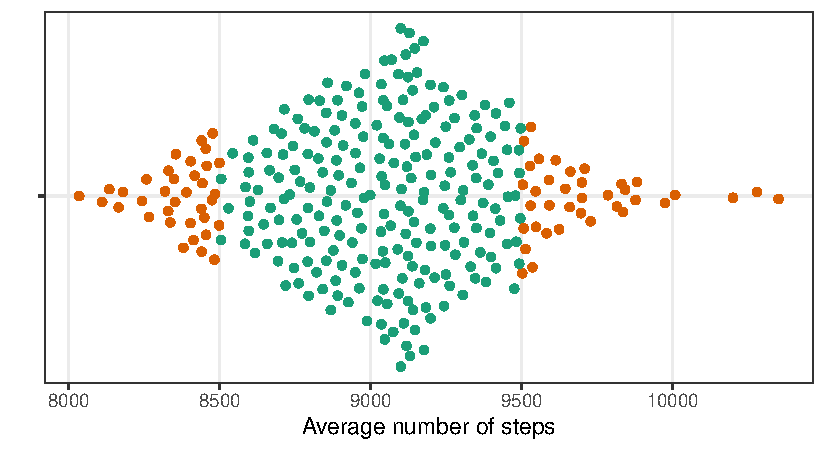
\includegraphics{index_files/figure-pdf/fig-step-count-1.pdf}

}

\caption{\label{fig-step-count}Number of days with fewer than 8,000
steps across 300 simulated 30-day periods. The orange bars indicate
instances where the count exeeds five days, representing an unexpected
outcome in this scenario.}

\end{figure}%

\section{Method}\label{sec-method}

\subsection{A workflow to assess the quality of unit
tests}\label{a-workflow-to-assess-the-quality-of-unit-tests}

In real-world applications, it is rare to create a set of unit tests can
fully guarantee expected results. On one hand, there is the cost of
effort involved in manually developing all these tests; on the other,
there is the inherent complexity of the problem. (can we - if we're
thriving for detecting 95\% of the cause?). However, the quality of unit
tests can be evaluated by simulated data. One set of tests is considered
better than another if a small set of tests can reliably detect
unexpected outcomes, which brings two criteria in the evaluation metric:
accuracy and parsimony. Figure~\ref{fig-metric-calc} illustrates the
workflow for calculating the metrics.

\phantomsection\label{cell-fig-metric-calc}
\begin{figure}[H]

\centering{

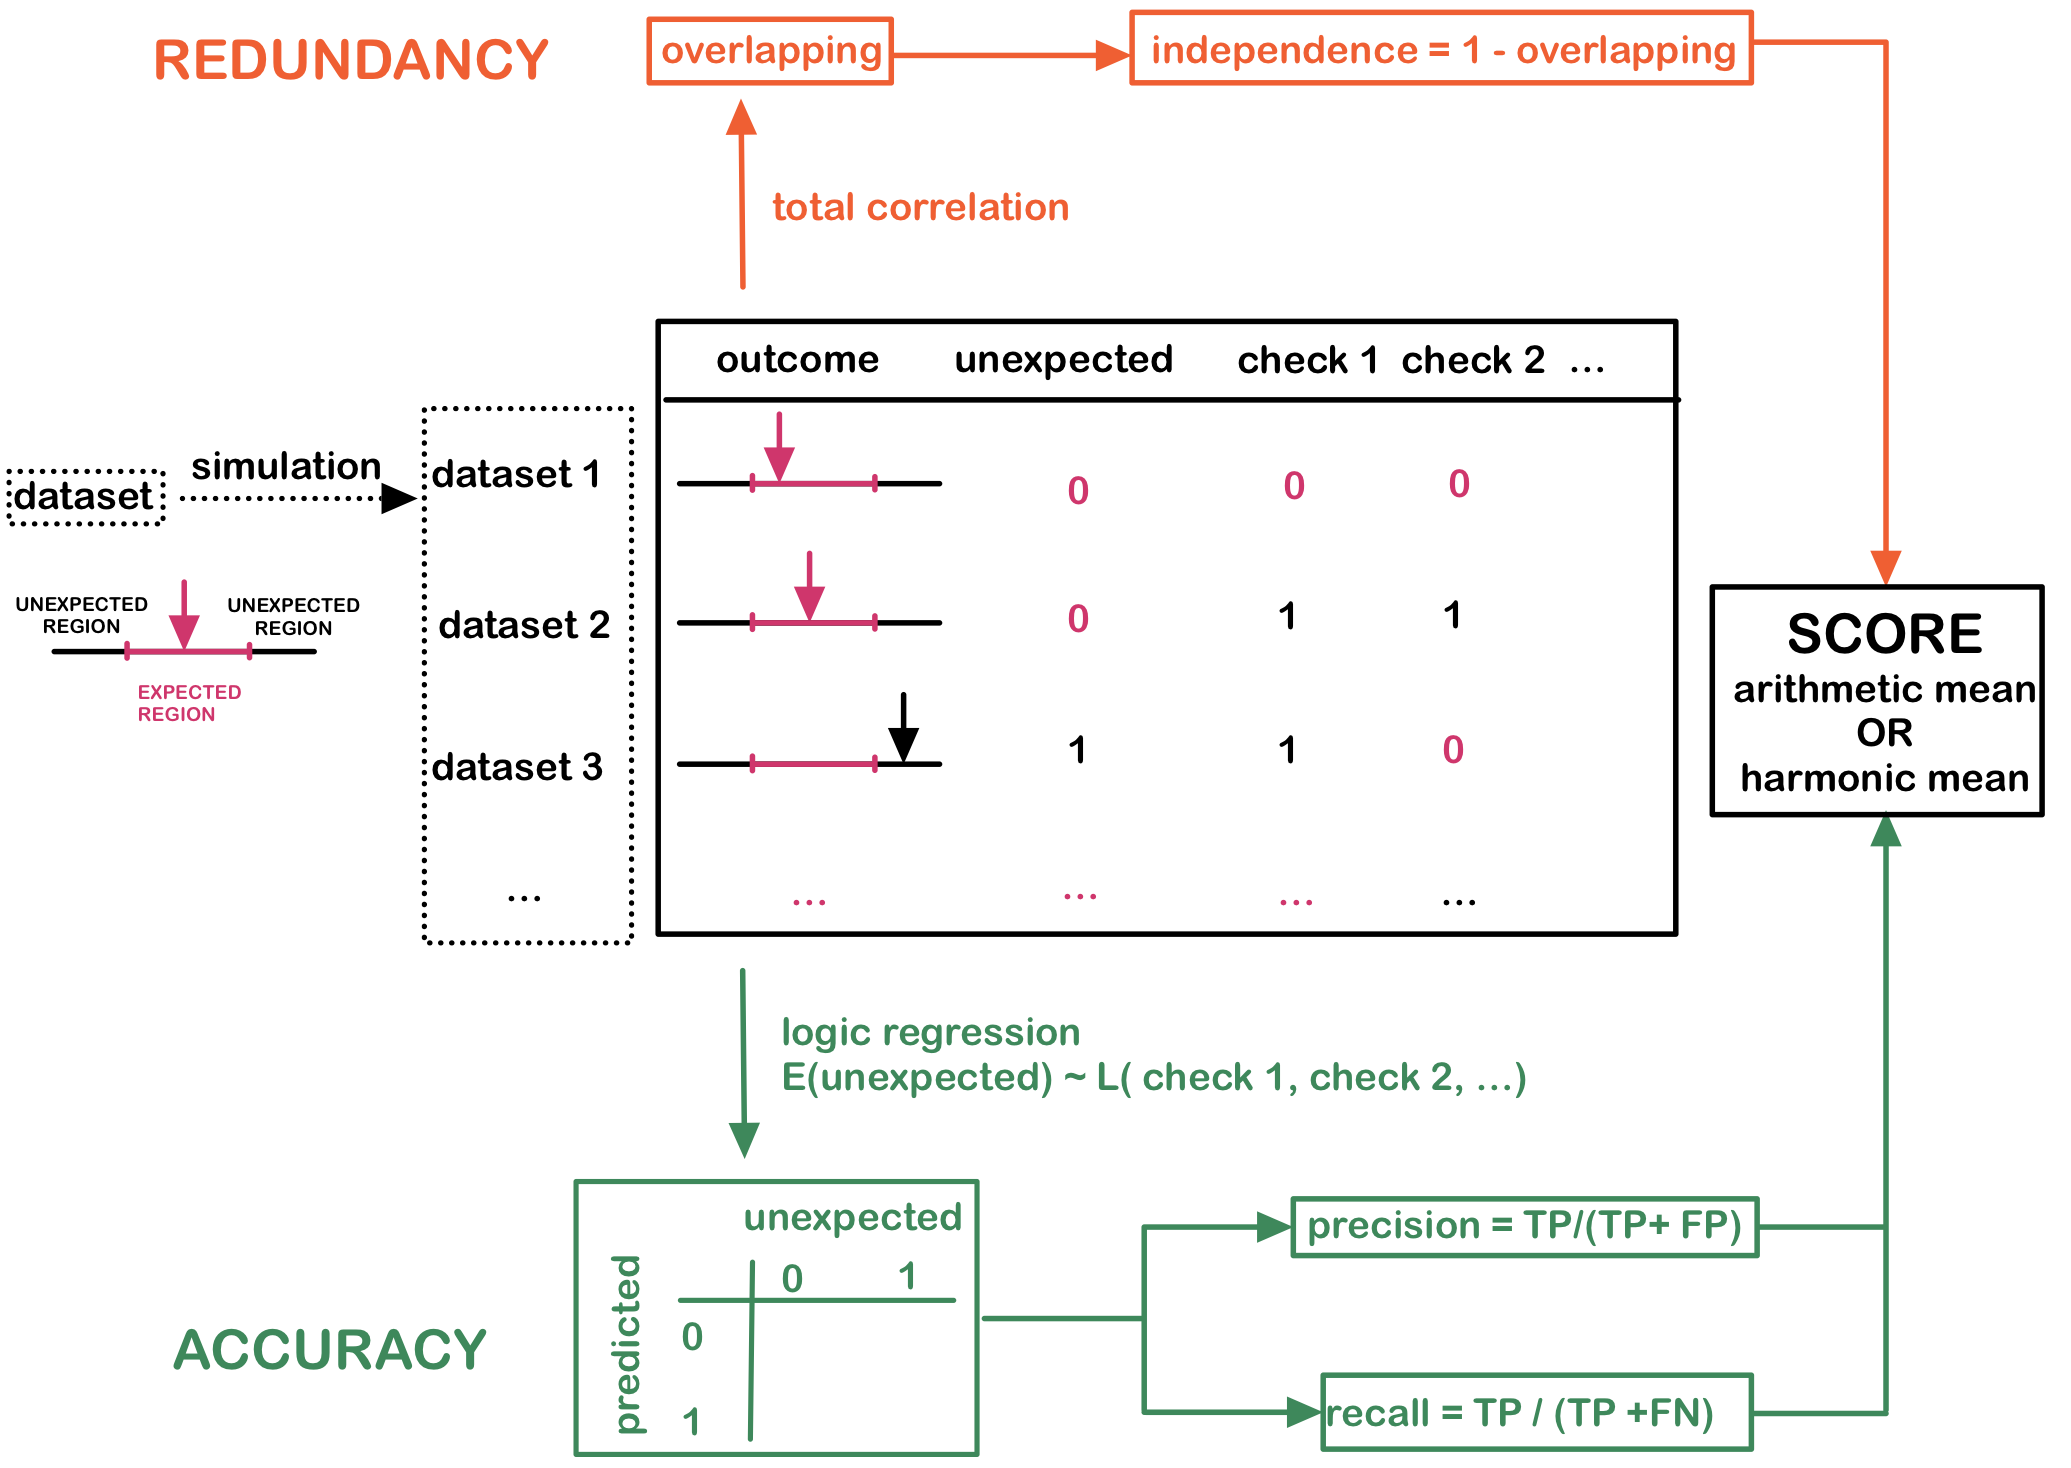
\includegraphics[width=6.73in,height=\textheight]{figures/metric-calc.png}

}

\caption{\label{fig-metric-calc}this is the cap}

\end{figure}%

Accuracy refers to a set of tests' ability to accurately detect
unexpected outcomes while minimizing false positives and false
negatives. A false positive can indicate (caution or skepticism on
checking the data), whereas a false negative suggests the tests may lack
sensitivity to unexpected outcomes. To model the relationship between
the plan and outcome expectation (binary-binary), a logic regression
model is used \citep{ruczinski_logic_2003}. Originally developed for SNP
microarray data, logic regression constructs Boolean combinations of
binary variables to solve regression problems {[}more introduction on
logic regression{]}. Compared to other tree-based methods or machine
learning methods for binary-binary prediction, logic regression produces
Boolean combinations, or meta rules, that combines unit tests to solve
the prediction problem. {[}need rewrite here{]}. The performance of the
tests can be evaluated using precision and recall metrics derived from
the confusion matrix of the logic regression prediction

\begin{itemize}
\tightlist
\item
  precision: the proportion of correctly identified unexpected results
  (true positives) out of all the predicted unexpected results (true
  positives + false positives)
\item
  recall: the proportion of correctly identified unexpected results
  (true positives) out of all the actual unexpected results (true
  positives + false negatives)
\end{itemize}

The second criteria is parsimony in the tests. While tests may score
high on accuracy, they may be less effective at explaining the reasons
behind unexpected results. This could happen if a set of tests are all
tangentially related to the cause of the unexpected results, but none
addressing the root cause. It may also occur if the tests are correlated
with one another, leading to redundancy.

To quantify redundancy, the concept of mutual information is used.
Mutual information \(I(x, y)\) measures the amount of information shared
between two random variables and is defined as the KL-distance
\(D(p \parallel q)\) between the joint distribution of the two variables
and the product of the marginal distributions:

\[I(x,y) = D\big(p(x,y) \parallel p(x)p(y)\big) = \sum_x \sum_y p(x,y) \log \frac{p(x,y)}{p(x)p(y)}\]

This concept extends naturally to multiple variables through total
correlation {[}ref{]}, \(C(X_1, X_2, \cdots, X_n)\), which captures
redundancy across a set of \(n\) variables:

\[C(X_1, X_2, \cdots, X_n) = \sum_{x_1} \sum_{x_2} \cdots \sum_{x_n} p(x_1, x_2, \cdots, x_n) \log \frac{p(x_1, x_2, \cdots, x_n)}{p(x_1)p(x_2) \cdots p(x_n)}\]

A high mutual information value indicates redundancy among the tests,
while a low value suggests that the tests are independent and provide
unique information to diagnose the unexpected outcome. To standardize
this measure, the total correlation \emph{per observation} is
calculated, and an independence score, ranging between 0 and 1, is
defined as 1 - mutual information.

To combine precision, recall, and independence into a single metric,
various mathematical means, such as arithmetic mean, harmonic mean, and
quadratic mean, can be used. The differences among these means are
minimal when the three metrics are similar. However, as the differences
among the metrics increases, the harmonic mean tends to produce the
smallest overall score, as it penalizes low values, while the quadratic
mean tends to produce the largest score by rewarding higher values more.
For simple interpretation of the score, the arithmetic mean is
preferred, while in applications where the difference between precision,
recall, and independence need to be penalized or rewarded more, the
harmonic and quadratic mean should be considered.

\subsection{Toy example revisited}\label{toy-example-revisited}

In the step count example, we can use the logic regression model to
evaluate the quality of the unit tests. The logic regression model is
fitted to the three unit tests (test1, test2, test3) and the outcome
expectation (unexpect) as the response variable. The model is then used
to predict the outcome expectation based on the unit tests. The
prediction is then compared to the actual outcome expectation to
calculate the precision and recall of the tests. The independence of the
tests is also calculated to assess the redundancy of the tests.
Figure~\ref{fig-logic-reg} presents the suggested logic regression model
as a combination of test 1 and test 3 with an OR operator.

Table~\ref{tbl-logic-reg} presents the calculated precision, recall, and
independence for the three individual tests and the combined test rule
(test1 OR test3) from the logic regression. The harmonic and arithmetic
means are included to evaluate the quality of the unit tests in
diagnosing unexpected step counts. The results show that the combined
test rule (test1 OR test3) has the highest precision, recall, and
independence, suggesting that it is the most effective test for
diagnosing unexpected step counts. We also include the metric calculated
from fitting a regression tree model to the data to compare the
performance of the logic regression model. The regression tree produces
a similar model of first split on test1 and then split on test3, and
results in the same accuracy and overall score as the logic regression
model.

top-down and bottom up (regression tree + logic tree): more naturally
useful summary of the say it is organized. (put down the plot)

\phantomsection\label{cell-fig-logic-reg}
\begin{figure}[H]

\centering{

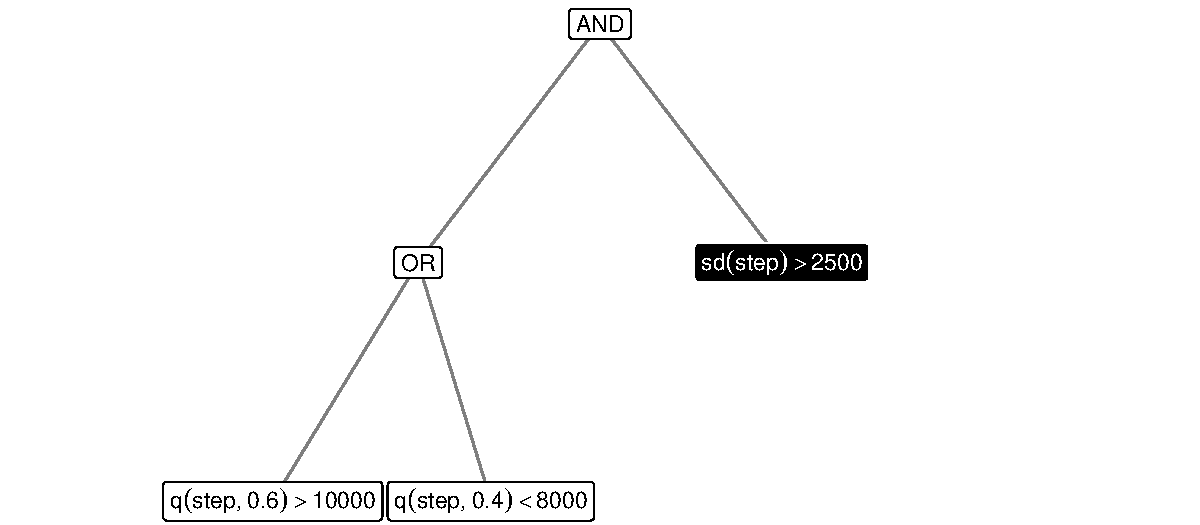
\includegraphics{index_files/figure-pdf/fig-logic-reg-1.pdf}

}

\caption{\label{fig-logic-reg}Logic regression model fitted to the three
unit tests (test1, test2, test3) and the outcome expectation (unexpect)
as the response variable. The model suggests using an OR rule to combine
test1 and test3 to predict the outcome expectation.}

\end{figure}%

\begin{longtable}[]{@{}
  >{\raggedright\arraybackslash}p{(\columnwidth - 10\tabcolsep) * \real{0.2424}}
  >{\raggedleft\arraybackslash}p{(\columnwidth - 10\tabcolsep) * \real{0.1515}}
  >{\raggedleft\arraybackslash}p{(\columnwidth - 10\tabcolsep) * \real{0.1061}}
  >{\raggedleft\arraybackslash}p{(\columnwidth - 10\tabcolsep) * \real{0.1970}}
  >{\raggedleft\arraybackslash}p{(\columnwidth - 10\tabcolsep) * \real{0.1364}}
  >{\raggedleft\arraybackslash}p{(\columnwidth - 10\tabcolsep) * \real{0.1667}}@{}}

\caption{\label{tbl-logic-reg}Accuracy (precision and recall) and
parsimony (independence) metrics for each individual unit test and for
the combined test rule (test1 OR test3) derived from the logic
regression model. The harmonic and arithmetic means of the three metrics
are included to evaluate the quality of the unit tests in diagnosing
unexpected step counts (more than five days with fewer than 8,000
steps).}

\tabularnewline

\toprule\noalign{}
\begin{minipage}[b]{\linewidth}\raggedright
tests
\end{minipage} & \begin{minipage}[b]{\linewidth}\raggedleft
precision
\end{minipage} & \begin{minipage}[b]{\linewidth}\raggedleft
recall
\end{minipage} & \begin{minipage}[b]{\linewidth}\raggedleft
independence
\end{minipage} & \begin{minipage}[b]{\linewidth}\raggedleft
harmonic
\end{minipage} & \begin{minipage}[b]{\linewidth}\raggedleft
arithmetic
\end{minipage} \\
\midrule\noalign{}
\endhead
\bottomrule\noalign{}
\endlastfoot
test1 & 0.482 & 0.964 & 1.000 & 0.730 & 0.815 \\
test2 & 0.214 & 1.000 & 1.000 & 0.450 & 0.738 \\
test3 & 0.589 & 0.805 & 1.000 & 0.762 & 0.798 \\
test1 OR test3 & 0.821 & 0.836 & 0.999 & 0.879 & 0.886 \\
regression tree & 0.821 & 0.836 & 1.000 & 0.879 & 0.886 \\

\end{longtable}

\section{Application}\label{sec-pm10-mortality}

A regression example is produced to illustrate the test selection
process for analyzing the effect of PM10 on mortality. The example
demonstrates how the procedure presented in Section~\ref{sec-method} can
be used to select cutoff values in the checks to diagnose an unexpected
PM10 coefficient from the generalized linear model.

Consider a generalized linear model (GLM) to study the effect of PM10 on
mortality {[}TODO: provide more context of the mortality-PM10 study{]}.
Analysts may expect a PM10 coefficient between {[}0, 0.005{]} after
considering the temperature confounding {[}TODO: reference{]}. This
expectation can be framed into a check that fails, labelled as 1, if the
PM10 coefficient is outside the range {[}0, 0.005{]}. Multiple factors
can impact the PM10 coefficient, such as the sample size, the strength
of the correlation between mortality and PM10, and the strength of the
correlation between mortality and temperature. Analysts may expect a
reasonable sample size to ensure the reliability of the coefficient
estimate. Outliers in the three variables can also leverage the
coefficient. While these are possible factors that could affect the
analysis result, it is not clear the cutoff values for these checks to
determine a failure. Here a list of checks are created in
Table~\ref{tbl-checks}.

\begin{longtable}[]{@{}l@{}}
\caption{A list of checks considered for the generalized linear model of
mortality on PM10 and temperature. The checks are based on the sample
size, correlation between mortality and PM10, correlation between
mortality and temperature, and univariate outlier detection. Multiple
cutoff values are specified for each check to determine a
failure.}\label{tbl-checks}\tabularnewline
\toprule\noalign{}
the check fails if \ldots{} \\
\midrule\noalign{}
\endfirsthead
\toprule\noalign{}
the check fails if \ldots{} \\
\midrule\noalign{}
\endhead
\bottomrule\noalign{}
\endlastfoot
Sample size less than or equal to 200 \\
Sample size less than or equal to 400 \\
Sample size less than or equal to 600 \\
Sample size less than or equal to 800 \\
Mortality-PM10 correlation less than -0.03 \\
Mortality-PM10 correlation less than -0.04 \\
Mortality-PM10 correlation less than -0.05 \\
Mortality-PM10 correlation less than -0.06 \\
Mortality-temperature correlation greater than -0.3 \\
Mortality-temperature correlation greater than -0.35 \\
Mortality-temperature correlation greater than -0.4 \\
Mortality-temperature correlation greater than -0.45 \\
Outlier(s) are presented in the variable PM10 \\
Outlier(s) are presented in the variable mortality \\
\end{longtable}

To generate replicate of the data, we first simulate the correlation
matrix of the three variables in a grid and then use a Gaussian copula
to generate a multivariate normal distribution based on the specified
correlation matrix and sample size. The multivariate normal distribution
is transformed using the normal CDF before the inverse CDF of the
assumed distributions of the three variables is applied. To determine
the appropriate distribution of each variable, various distributions are
fitted and compared. This includes poisson and negative binomial for
mortality; gamma, log-normal, exponential, weibull, and normal for pm10
and temperature; and beta for pm10 after rescaling the data to
\([0-1]\). AIC is used to determine the best distribution fit for each
variable with qq plot presented in Figure~\ref{fig-dist-fit} to evaluate
the fit. AIC suggests a negative binomial distributio nfor mortality, a
beta distribution for PM10 (multiple by 100 to obtain the original
scale), and a Weibull distribution for temperature. To include the
effect of outlier, we add a single outlier to the data for mortality and
PM10 {[}more details{]}.

\phantomsection\label{cell-fig-dist-fit}
\begin{figure}[H]

\centering{

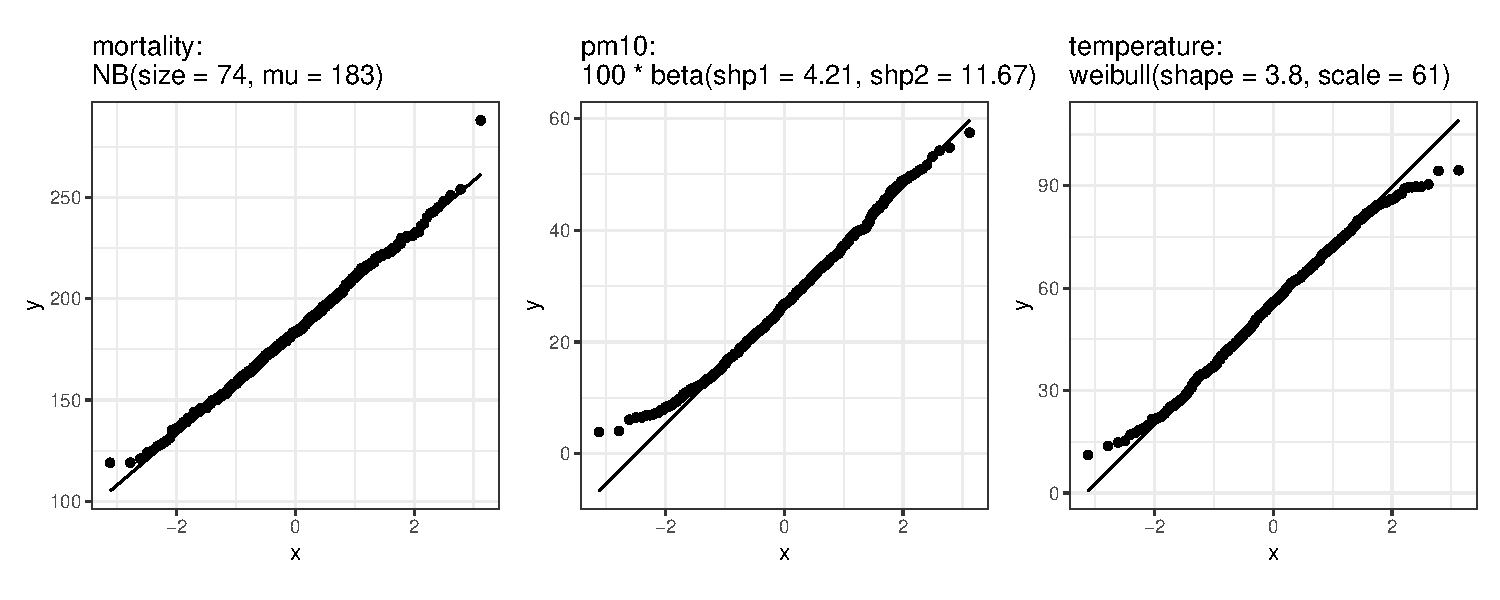
\includegraphics{index_files/figure-pdf/fig-dist-fit-1.pdf}

}

\caption{\label{fig-dist-fit}QQ-plot of the distribution fit for
mortality, PM10, and temperature based on the fitted distribution from
the original data. The fitted distribution is compared to the observed
data to assess the distribution fit.}

\end{figure}%

\begin{figure}

\centering{

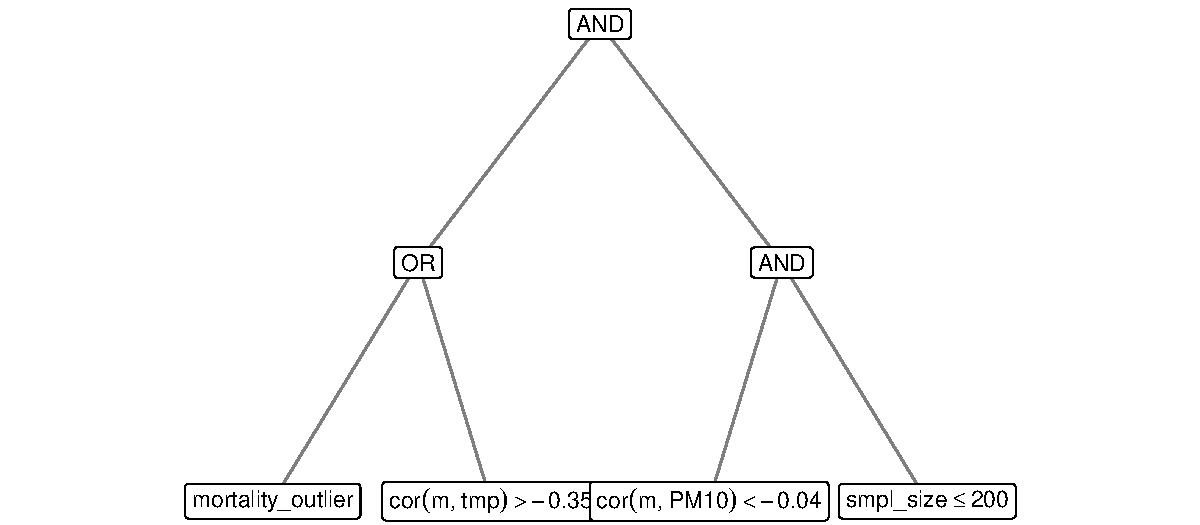
\includegraphics{index_files/figure-pdf/unnamed-chunk-8-1.pdf}

}

\caption{\label{fig-linear-reg-tree}Logic regression model fitted to the
twelve unit tests and the outcome expectation (unexpect) as the response
variable. The model suggests the relationship:
(\(\text{cor}(\text{m}, \text{tmp}) > -0.35\) AND
\(\text{smpl\_size} \le 600\)) OR
\(\text{cor}(\text{m},  \text{PM10}) < - 0.05\)}

\end{figure}%

\begin{longtable}[]{@{}
  >{\raggedleft\arraybackslash}p{(\columnwidth - 12\tabcolsep) * \real{0.0882}}
  >{\raggedleft\arraybackslash}p{(\columnwidth - 12\tabcolsep) * \real{0.1471}}
  >{\raggedleft\arraybackslash}p{(\columnwidth - 12\tabcolsep) * \real{0.1029}}
  >{\raggedleft\arraybackslash}p{(\columnwidth - 12\tabcolsep) * \real{0.1765}}
  >{\raggedleft\arraybackslash}p{(\columnwidth - 12\tabcolsep) * \real{0.1912}}
  >{\raggedleft\arraybackslash}p{(\columnwidth - 12\tabcolsep) * \real{0.1324}}
  >{\raggedleft\arraybackslash}p{(\columnwidth - 12\tabcolsep) * \real{0.1618}}@{}}

\caption{\label{tbl-linear-reg}Accuracy (precision and recall) and
parsimony (independence) metrics derived from the logic regression
model, along with harmonic and arithmetic means, for individual unit
tests (1: sample size, 2: mortality-PM10 correlation, 3:
mortality-temperature correlation), and the combined test rule 4:
(sample size AND mortality-temperature correlation) OR mortality-PM10
correlation.}

\tabularnewline

\toprule\noalign{}
\begin{minipage}[b]{\linewidth}\raggedleft
tests
\end{minipage} & \begin{minipage}[b]{\linewidth}\raggedleft
precision
\end{minipage} & \begin{minipage}[b]{\linewidth}\raggedleft
recall
\end{minipage} & \begin{minipage}[b]{\linewidth}\raggedleft
overlapping
\end{minipage} & \begin{minipage}[b]{\linewidth}\raggedleft
independence
\end{minipage} & \begin{minipage}[b]{\linewidth}\raggedleft
harmonic
\end{minipage} & \begin{minipage}[b]{\linewidth}\raggedleft
arithmetic
\end{minipage} \\
\midrule\noalign{}
\endhead
\bottomrule\noalign{}
\endlastfoot
1 & 0.087 & 0.215 & 0 & 1 & 0.175 & 0.434 \\
2 & 0.988 & 0.610 & 0 & 1 & 0.822 & 0.866 \\
3 & 0.392 & 0.581 & 0 & 1 & 0.569 & 0.658 \\
4 & 0.649 & 0.641 & 0 & 1 & 0.732 & 0.763 \\
5 & 0.760 & 0.880 & 0 & 1 & 0.869 & 0.880 \\

\end{longtable}

A logic regression is fitted to predict whether the PM10 coefficient is
unexpected (outside the range of {[}0, 0.005{]}) using the checks listed
in Table~\ref{tbl-checks}. Precision, recall, and independence score,
along with their harmonic and arithmetic mean are calculated.
Figure~\ref{fig-linear-reg-tree} shows the logic regression tree from
the fitted model and Table~\ref{tbl-linear-reg} prints the numerical
summary of four selected single test and their combined test found by
the logic regression. The logic regression model picks up the following
cutoff value for each type of check:

\begin{itemize}
\tightlist
\item
  sample size \emph{larger than} 200
\item
  mortality-temperature correlation greater than -0.35
\item
  mortality-PM10 correlation less than -0.04
\item
  mortality contain outliers that are detected by the univariate outlier
  detection
\end{itemize}

The tree structure suggests checking mortality-PM10 correlation and a
sample size larger than 200 with an additional check of either outlier
on mortality or correlation between mortality and temperature. This
combined check rule generates a 0.76 precision and a 0.88 recall for
predicting the unexpected PM10 coefficient. The single check,
\texttt{cor(m,\ PM10)\ \textless{}\ -0.03}, is also powerful with a high
precision of 0.988, but the low recall value of 0.61 suggests its high
false positive rate, as compared to the combined rule suggested by the
logic regression.

\section{Discussion}\label{sec-discussion}

TODO

\begin{itemize}
\item
  how to systematically simulate data is still unknown
\item
  plotting is a critical way to check data and they can still be frame
  into checks. i.e.~the density/ histogram suggests there are outliers.
  It is a open problem to how to encode the visualization into checks.
\item
  currently no automated way to generate checks. It is interesting to
  see how check generation can be automated, although it requires the
  inputs from experts across a wide array of common scenarios.
\item
  checks are also closely related to the concept of unit tests in
  software engineering. While unit tests are designed to isolate and
  test specific aspects of the code, it is difficult for analysis
  validation check to do so.
\item
  There are cost and benefit on setting expectation on different
  granularity. At the lowest level, one may have a plan for each data
  entry and every data handling steps. This requires more work from the
  analysts and may not be practical in practice. For more complex
  analyses, analysts may divide the analysis into sections and set
  expectations for each. They can then focus on the specific sections
  flagged by the tests and sub-divide the sections to set expectation
  and diagnose the analysis in a hierarchical manner.
\end{itemize}

\section{Conclusion}\label{sec-conclusion}

TODO

\section{Acknowledgement}\label{acknowledgement}

The article is created using Quarto \citep{Allaire_Quarto_2022} in R
\citep{R}. The source code for reproducing the work reported in this
paper can be found at:
\url{https://github.com/huizezhang-sherry/paper-avc}.


\renewcommand\refname{References}
  \bibliography{references.bib}



\end{document}
